

\documentclass[12pt]{article}
\usepackage[T1]{fontenc}
\usepackage[utf8]{inputenc}
\usepackage{amsmath}
\usepackage{microtype}
\usepackage{listings}
\setlength{\parindent}{0pt}
\usepackage{fancyvrb}
\usepackage{enumerate}
\usepackage{array}
\usepackage[breaklinks=true,linktocpage,hidelinks]{hyperref}
\usepackage[letterpaper]{geometry}
\usepackage{url}
\usepackage{graphicx}
\usepackage{fullpage}

\usepackage{pgfplots}
\usepackage{pgfplotstable}
\usepackage{tikz}

\usepackage{fancyhdr}
\usepackage{fancybox}
\usepackage{multicol}
\usepackage{xcolor}
\usepackage{adjustbox}

\pgfplotsset{compat=newest}
\usetikzlibrary{shapes,backgrounds,arrows}
\usepgfplotslibrary{external} 

\definecolor{brewcol1}{RGB}{166,206,227}
\definecolor{brewcol2}{RGB}{31,120,180}
\definecolor{brewcol3}{RGB}{178,223,138}
\definecolor{brewcol4}{RGB}{51,160,44}
\definecolor{brewcol5}{RGB}{251,154,153}
\definecolor{brewcol6}{RGB}{227,26,28}
\definecolor{brewcol7}{RGB}{237,179,1}
\definecolor{brewcol8}{RGB}{202,178,214}
\definecolor{brewcol9}{RGB}{206,27,1}

\geometry{hmargin=1.87cm, vmargin=1.87cm}
\bibliographystyle{siam}

\DeclareTextFontCommand{\helvetica}{\fontfamily{phv}\selectfont\small}


\begin{document}

\clearpage\thispagestyle{empty}
\begin{center}
\textbf{Difficult transition for sugar maple in Boreal forest under climate change? \\
Impact of alternative stable states on Sugar maple migration.}
\vskip 2em
Research proposal
\vskip 1em
Master in Wildlife management
\vfill
By
\vfill
Steve Vissault 
\vfill 
For
\vfill
\textbf{Richard Cloutier}, Pr.\\
Director of the program committee
\vskip 2em
\textbf{Dominique Arsenault}, Pr.\\
President of the jury
\vskip 2em
\textbf{Matt Talluto}, PhD\\
Research Co-director
\vskip 2em
\textbf{Dominique Gravel}, Pr.\\
Research Director
\vfill
\vfill
Université du Québec à Rimouski\\
\today

\end{center}

\newpage
\setcounter{page}{1}

\section{Introduction}

\textbf{Context.}  The boreal region is warming twice as fast as the global
average and  this will inevitably alter the species composition in boreal
forests \cite{Scheffer2012,Hughes2000}. Sugar maple (\textit{Acer saccharum})
is a widespread and abundant tree in north-eastern North America and is one of
the most representative species of northern temperate forests
\cite{Graignic2013,Messaoud2007,Kellman2004,Barras1998}. This species is one
of the species expected to migrate northward towards the northern limit of the
temperate forest \cite{McKENNEY2007,Goldblum2005}. Predicting shifts in the
range of sugar maple under climate change is an important challenge because
this species is highly desirable by hardwood and maple syrup producers, two
large economic sectors in Quebec. The expected northward migration of sugar
maple and the associated community during climate change will increase the
ecotone between the boreal and temperate forest of Québec.\\

Some species mostly representative of northern forest ecosystems are predicted
to expand their distribution range broadly to the north. As an example, sugar
maple is expected to move northward closed to the Ungava bay
\cite{McKENNEY2007}. These predictions are built on species distribution
models based only on climatic conditions though maple regeneration depends
both on macroclimatic (\textit{i.e.} regional climate) and microclimatic
conditions (\textit{i.e.} soil conditions). Thus, the expansion of this
species distribution is difficult to predict because microconditions
(\textit{e.g.} soil moisture, pH) can mitigate macroconditions such as global
warming \cite{DeFrenne2013}. Even if the regional climate conditions are
favorable \cite{Kellman2004}, the microconditions found in the boreal forest
could affect the establishment of sugar maple
\cite{Kellman2004,Moore2008,DeFrenne2013,Barras1998}. For instance, in boreal
forest, colder temperatures from shading and excess soil moisture due to snow
melt cause litter to be more acidic and fibrous during the spring  when the
seeds are supposed to be germinating (\textbf{Source}). The maple could then
be unable to migrate in boreal forests as a result of negative local
feedbacks. Thus, the landscape structure could be seen as a patchy mosaic
structure where stand soil conditions are driving the spatial occurences of
boreal and temperate species stands despite a regional climate favorable to
temperate species. In this case, boreal and temperate stands are two
alternative stable states, \textit{i.e.} contrasted states occuring in the
same climate conditions \cite{scheffer2009critical}. This situation generate a
tension between the boreal and temperate forest meaning that soil
perturbations can produce drastic shift in community composition in the
boreal-temperate forest ecotone.\\

% DG: be careful to use constant terminology, avoid switch between terms, such as macroclimate and regional climate. Define all terms.


\textbf{Objectives.} The main objective of this project is to investigate the
transition  between the boreal and temperate forests under different climate
change and forest management scenarios.In this context, we will test two
different hypothesis: ($H_1$) Alternative stable states are occuring in the
boreal- temperate forests ecotone;  ($H_2$) Time lags in the response to
climate change will be larger in areas where alternative stable states are
occuring. In order to achieve my general objective and test these hypotheses,
I will (1) develop a climate-dependent model of state transition (STM)
representing the dynamics of the boreal and temperate trees; (2) investigate
the spatial structure of maple distribution and the occurrence of alternative
stable states in the transitional zone; and finally (3) run simulations of
maple migration under different climate change scenarios. \\

The first section of this proposal reviews the context of the study. The first
part of the review presents the concept of alternative stable states and
critical transitions in ecosystem properties. The second part focuses on sugar
maple, its associated community in the temperate biome and a justification
about why alternative stable states are expected to occure at the boreal-
temperate forests ecotone. The second section of this document describes the
model and the methodology that I will employ to fill my specific  objectives.
To conclude, the last part presents the general timeline associated with this
project.

\section{Review} 

\begin{figure}[t]
	\begin{center}
	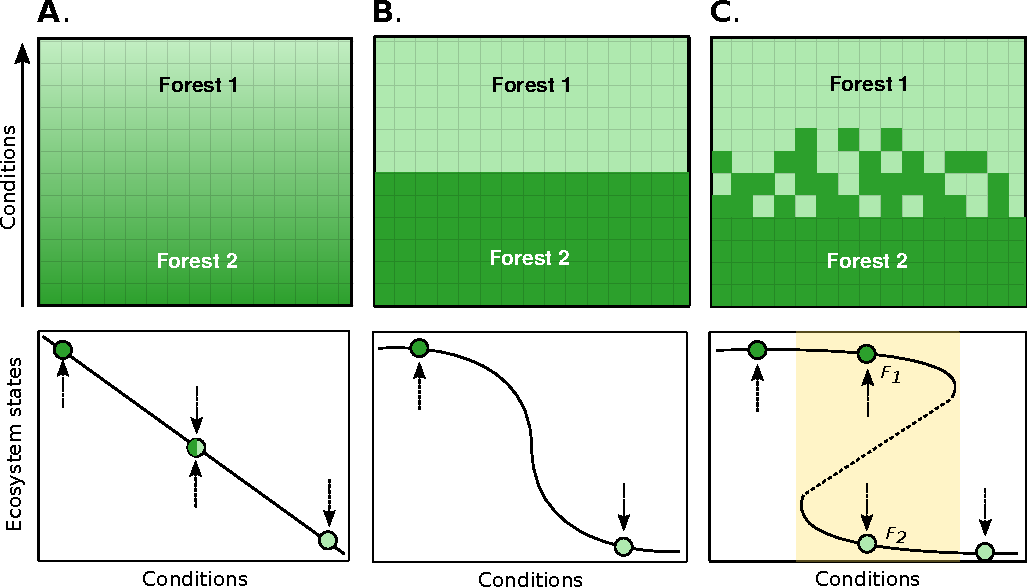
\includegraphics[width=0.8\textwidth]{fig/states.pdf}
	\end{center}
	\caption{Schematic representation of different ways in which the equilibrium
	states from forest-forest system can vary over climatic gradients such as temperature, precipitation
	or soil moisture. Three differents responses are presented,
	\textbf{(A)} gradual, \textbf{(B)} basic fold, \textbf{(C}) catastrophic fold.
	The first line illustrates a conceptualization of a transitional landscape
	between the boreal (light green) and the nordic temperate forests (dark
	green). The second line presents the stable states rise by the forest
	given a specific environnemental condition. Arrows indicate the
	direction the system moves if not at the equilibrium. Solid lines represent stable states along the boreal-temperate
	transition, and the dashed line (in yellow highlight) unstable equilibrium. This zone,
	called hysteresis, is particulary unstable and small fluctuations in
	environnement conditions give rise to a contrasted state representing an
	alternative stable states. ($F_1$ or $F_2$).}
	\label{fig1}
\end{figure}

%%%% Travailler davantage sur la théorie pas trop d'exmple (travailler sur la senconde ligne des figures).
%%% L'exmple vient avec l'étude du système naturelle dans la seconde section. 
%% Qu'est ce qui génère états stable alternatifs ? Système non linéaire, Dynamic rétroactive très forte.

\textbf{Alternative stable state in forest ecosystems.} Many empirical and
modeling studies have been conducted on the transition between forest to non-
forests (e.g. Boreal-Tundra)
\cite{Scheffer2012,Scheffer2001,Hirota2011,Messaoud2007} but little attention
has been given to evaluate the forest-forest ecotone
\cite{Goldblum2010,Graignic2013}. At landscape scale, transition between  the
temperate and boreal forests can be approached as a dynamical system where
each forest biome is a stable state. The occurrence of different states at a
location or a time depends on environmental conditions (e. g. soil,
temperature) driving the dynamics. When a small environmental change occur,
most dynamical systems respond almost linearly, with no threshold leading to
drastic changes in the ecosystem functionning (Figure \ref{fig1}.a)
\cite{Scheffer2001,Scheffer2009}. In this case, ecosystem states can be seen as a
continuum along the environnemental gradient
\cite{Scheffer2001,Scheffer2009,scheffer2009critical}.


For instance, when the annual precipitation increase slightly in a forest
deciduous stand, the new local condition gives rise to a favorable new species
establishment. Another type of response
occurs more frequently in nature.
%%%%% Travailler cet example (peut être même l'abandonner)
%DG: you said above that most system respond linearly, it is thus not possible that abrupt changes are more frequent...

Such systems are insensitive to small change in environmental conditions over
certain ranges but respond strongly when a threshold is reached (Figure
\ref{fig1} .b) \cite{scheffer2009critical}. For instance, tree mortality can
increase sharply when a toxin is added to the environment.
\cite{scheffer2009critical}. In this case, the response curve of the natural
systeme is not linear but lightly folded and a small change can drive the
sytem to a treshold and lead to major changes. Small changes in the initial
conditions can transform abruptly the community composition and lead to a
sharp spatial division between states (Figure \ref{fig1}.c, upper line). Lastly, the
response curve can be folded backwards and alternative stable states could
occur (Figure \ref{fig1} .c).  When the environmental conditions approach a
tipping point on the folded upper branch, the system cannot pass smootly to
the lower branch. Small forcing on initial condition of the state $F_1$
transfer immediatly the system into a contrasted state $F_2$ (Figure
\ref{fig1} .c). This point is called a \textit{Bifurcation point} and a small
forcing on those critical states can drive the system into backward or forward
shifts.

% dg: the definition should come a couple of sentence above.

In this situation, the system present alternative stable states who mean the
presence of contrasted states over certain range of environmental conditions
\cite{scheffer2009critical}. An intermixed of constrasted patches in a ecotone
landscape is expected in the area of bi-stability \ref{fig1} .c (upper part).
This layout could be easily applied to the hardwood-boreal forest patchiness
structure often attribute to differences in soils, nutrient status and
topographical factors \cite{Society2014}.\\

%DG: this whole paragraph has a strange structure, mixing the theory, examples and then references to your hypothesis. I wonder if you should not put aside the boreal-temperate case for this paragraph since you haven't presented yet your main hypothesis

\textbf{Natural system studied.} There is no distinct boundary at the boreal-
temperate ecotone. A broad transition zone exists where stands of coniferous
deciduous species co-occur at the regional scale \cite{Goldblum2010}. A
macromosaic landscape can be observed with pure stands of deciduous trees on
favorable sites and pure coniferous stands on less favorable sites
\cite{Goldblum2010}. 

% Defined what we mean by "favorable" ?

This segregated patches distribution could be explain by
the fact than microclimatic conditions can modulate establishement of those
forests \cite{DeFrenne2013}. Distribution of deciduous and boreal forests
within the ecotone is not determined by macroclimatic conditions, but rather
by local variation of substrate, drainage, physical soil properties, and
nutrient avaiblity \cite{Goldblum2010,Society2014}.  For instance, balsam fir
(\textit{Abies balsamea}) is often related to deep organic horizons and
coarse xeric deposits, while sugar maple is mostly present in opposite edaphic
conditions \cite{Messaoud2007,Kellman2004,Barras1998}.

%DG: strange wording, should'nt be the opposite, ie that specific conditions are associated (consequent) to tree composition?

Moreover, boreal and hardwood forests are dominated by trees of distinctive
physiognomy, which is expected to produce distinctive litter and light
micro-environments \cite{Barras1998}.

A positive feedback contribute to the mainetance of the community type if the
dominant tree species promotes conditions facilitating its own regeneration
\cite{Barras1998}. Frelich \textit{et al.}(1993) \cite{Society2014}
hypothesized that sugar maple is subject to such a feedback.  Knowing this,
the alternative stable states is a relevant framework to study this ecotone
dynamic because the soil conditions and role of dominant species in
regeneration seems to act as main feedbacks on the temperate forest
establishment generating a patchiness landscape (Figure \ref{fig1}.c, upper
panel).

%DG: reword the previous sentenc, unclear

In this context, we expected to find patch dominated by boreal species and
others dominated by temperate species under a certain range of climatic
conditions. Thus, the soil condition and the role of dominant species in
boreal and temperate forest need to be investigate as main drivers in
alternative stable states
\cite{Kellman2004,Moore2008,DeFrenne2013,Barras1998}.

%MT: Good summary. You might come back to climate change here, as well, to remind the reader that you will also be testing some hypotheses about climate change.
%DG: not clear what you mean at the previous sentence.

% We used maple sugar basa areal in function of black
% spruce, white spruce and balsam fir basal area to compute the relative
% abundance of sugar maple. Given the above statements, we used mainly two
% climatic variables (annual mean temperature and annual precipitation) to
% identify the alternative stable states present in the boreal-temperate
% ecotone. The relationship was performed on climatic variables and sugar maple
% relative abundance using kernel density plot function. We obtained the
% probability of observed a sample plot as function of sugar maple relative
% abundance and mean annual temperature (Figure \ref{fig1}). In both case,
% alternative stable states are presents whereas the function graphed has a
% bimodal distribution. At low precipitation or temperature conditions, the
% probability of observing a parcel sampled without sugar maple is higher than
% intermediate climatic conditions where the multimodal distribution appear. The
% density function suggest the presence of alternative stabe states  in response
% of intermediate climatic conditions: one state wherein sugar maple dominates
% and an another in which sugar maple is absent. \\

\section{Methods}   

\begin{wrapfigure}{L}{0.45\textwidth}         
	
\begin{center}
	
				\tikzstyle{noeud}=[circle,
				                  thick,
				                  minimum size = 1.5cm,
				                  inner sep =5pt,
				                  draw=brewforest3,
				                  fill=brewforest1]
				\tikzstyle{noeud2}=[circle,
				                  thick,
				                  minimum size = 1.5cm,
				                  inner sep =5pt,
				                  draw=brewforest3,
				                  fill=brewforest3]
				\tikzstyle{noeud3}=[circle,
				                  thick,
				                  minimum size = 1.5cm,
				                  inner sep =5pt,
				                  draw=brewforest3,
				                  fill=brewforest3]
	
				\begin{tikzpicture}[->,>=stealth',auto,scale=0.65]
				      \node [circle,noeud2] (M) at (0,0) {\color{white}\textbf{M}};
				      \node [circle,noeud2]  (C) at (-5,5) {\color{white}\textbf{C}};
				      \node [circle,noeud2] (D) at (5,5) {\color{white}\textbf{D}};
				      \node [circle,noeud2] (T) at (0,10) {\color{white}\textbf{T}};
	
						\draw[thick,-latex] (M) to[bend right=10] node[above,sloped] {$S_C$} (C);
						\draw[thick,-latex] (C) to[bend right=10] node[below,sloped] {$\beta_d \cdot (D+M)$} (M);
	
						\draw[thick,-latex] (D) to[bend right=10] node[above,sloped] {$\beta_c \cdot (C+M)$} (M);
						\draw[thick,-latex] (M) to[bend right=10] node[below,sloped] {$S_D$} (D);
	
						\draw[thick,-latex] (D) to[bend right=10] node[above,sloped] {$e$} (T);
						\draw[thick,-latex] (T) to[bend right=10] node[below,sloped] {$\phi_D$} (D);
	
						\draw[thick,-latex] (T) to[bend right=10] node[above,sloped] {$\phi_C$} (C);
						\draw[thick,-latex] (C) to[bend right=10] node[below,sloped] {$e$} (T);
	
						\draw[thick,-latex,transform canvas={xshift=0.8ex}] (T) to node[above,sloped,rotate=90,transform canvas={xshift=3ex}] {$\phi_M $} (M);
						\draw[thick,-latex,transform canvas={xshift=-0.8ex}] (M) to node[above,sloped,rotate=-90,transform canvas={xshift=-3ex}] {$e$} (T);
				\end{tikzpicture}
	\end{center}	


	\caption{Conceptual representation of the transition model between deciduous ($D$),
	mixed ($M$) and coniferous ($C$) stands. $T$ corresponds to a transitionnal state. 
	Perturbations, natural and anthropogenic,  occur with a frequence $e$. Parameters $\beta$
	and $S$ are rates of colonisation and succession,
	respectively. We define the recovery rates ($\phi_c$ et $\phi_d$) as $\phi_c
	= \alpha_c \cdot (M+C) \cdot [1- \alpha_d \cdot (D +M)]$ and $\phi_D =
	\alpha_d \cdot (D+M) \cdot [1- \alpha_c \cdot (C +M)]$, to finaly get this
	equation $\phi_m = \phi_c \cdot \phi_d$. 

%MT: I am not sure I follow this

	The parameter $\alpha$ represents the 
	recovery rate after a patch has been disturbed.}         
	\label{Model}
\end{wrapfigure}

In this section I first describe the  model representing dynamics at the
boreal-temperate ecotone. Secondly, I present the  data that will be used to
parametrize the model.

%DG: reword the following sentence, way too convoluted! Write simple, straight

Whereas the transition between temperate and boreal forests is influenced by
environnemental conditions and proportion of coniferious and deciduous
available in the neighbourhood, the third section section will dedicated on
those factors and their parametrization. The last section describes the
simulation and validation techniques.\\

%MT section : I don’t think this is necessary. These sorts of summaries can be useful for long works, but this proposal is very short, so your reader is not likely to forget where you are going.

%DG: validation should come before the simulations. You validate the model to make sure the parameterization is ok, then you run the simulations
%DG: you must also explain how you define the states: by the composition of the dominant species?


\textbf{Model description.} The model represents the transition probability
between four different forest states: \textbf{(D)} Deciduous, \textbf{(M)}
Mixed and \textbf{(C)} Coniferous (Figure \ref{Model}).

%DG: what spatial scale is a single spatial unit?

Disturbances is an important driver of forest dynamics (e .g. Fire in boreal
forest or frost in temperate forest). When gap event occur in deciduous patch,
species presents will be replaced by shade intolerant species as aspen and
white birch, well adapted to the new shading condition.

%MT: If you are targeting a general audience, you will have to explain what you mean by a “gap event”
%DG: hold on, what type of disturbance are you talking about? At some point you'll have to define the spatial scale of interest for a given patch because the disturbance could either represent major or minor events, but not both. 

Disturbances  integrated within the model across the transitional patch
\textbf{(T)} (Figure \ref{Model}).

%DG: badly worded, you mean that the transition state could only occur following a disturbance. but disturbances could also lead to non transitional states. 

Dominance by late-succesional species are responsible for a transition from
state T to other states (C, D or M). Transitions between all states are
possible  except the direct transition between a deciduous and coniferous
stands, which does not occur because it systematically require an intermediate
step in state M.

%DG: you will have to read again and again this description of the model, it has to be crystal clear becaus it is so fundamental. 

%DG: at some point you will need to say that the transitions are climate-dependent.

For exemple, when a coniferous patch $C$ has been disturbed, a rate $e$, this can be
recovered to another state following $\phi_c$. 

%DG: always mention that the transition from X to Y
% MT: This wording is very confusing. From the figure, the parameter you mention is the rate of changing from T to C, but that is not what you are saying here. 

This term is taking in account a specific patch recovery rate ($\alpha_{c}$),
the availability of coniferous species ($M+C$) and the proportion of patches
unconverted into a deciduous state ($1- \alpha_d \cdot (D +M)$).

%DG: last part of the sentence not clear, reword.
%MT: Also confusing - alpha is not in the figure. Also, why is phi aggregated, when other rates are not? Why use phi when it is really a function of other parameters, and is dynamic. In fact, the terminology is incorrect, since phi is a function, not a parameter - it will change based on the availability of different patch types on the landscape.
%MT: Previously, you said phi depends on M+C, but here it is D+M. Which is correct?

The dynamics of state $T$ is described by the differential equation:
$\frac{\delta T}{\delta t} = e \cdot (C+M+D) - T \cdot (\phi_d + \phi_c +
\phi_m)$. If a patch $C$ is undisturbed, deciduous species $(D+M)$ can spread
over the patch at a rate $\beta_d$. Mixed stands $M$ turn into coniferous
stands at a rate $S_c$.  The dynamic of coniferous states is described by the
differential equation $\frac{\delta C}{\delta t} = \phi_C \cdot T + S_c \cdot
M - \alpha_d \cdot (D+M)\cdot C - e \cdot C$. 

%MT: I think these equations will need more description, and it will need to be very clear. Also, why only present T and C? Where are the other two?

The model is spatially implicit and assume that all space is occupied by one
state, so that the proportions of land cover occupied by all types of patch
sum to 1. 

%MT: I don’t understand this. How is all space occupied by a single space? There must be variance for it to be an interesting mode

The model will be solved at equilibrium to understand if alternative
stable states are possible and under which conditions.\\

%MT: To what end? What is the purpose of this step?. In order to be include in C++

\textbf{Data description.} The parameterization and validation of the model
will be conducted using the QUICC-FOR\footnote{Quantifying and mapping impact
of climate change on the forest productivity in eastern Canada.} database
containing large permanent (PP) and temporary (PT) sample plots from
United States and Canada. Data are freely provided by partners. They and
covering 3 eastern Canadian provinces (\textit{ca.} 16,000 plots) and 31 states of
eastern USA (\textit{ca.} 50,000 plots). Surveys started in the 1970s and includ up to
5 remeasurements, with the interval between sampling ranging from 5 to 10
years. Data is recorded for seedlings, trees, saplings and stand level. Stem-
level information including diameter at breast height (DBH), species, state of
the stem (e. g. alive or dead), height, age and canopy position. Seedling and
sapling data provide numbers of individuals by class of DBH and species. The
stand-level data include many relevant informations about soil deposit,
drainage, disturbances, cover type and, age and height of the stand. All plot
inventories are geo-referenced. For each plot location, some climatic
variables are include and extract by interpolation from the climatic model
ANUSPLIN \cite{McKenney2011}. We will parameterize the model using annual
rainfall (mm) and average temperatures (\ensuremath{^\circ}C) of the previous
30 years the year of the plot sampling. 

%MT: This is an awkward transition into the climate data, and might just warrant a new paragraph. Some earlier hypotheses with respect to climate will also help the reader remember why these data are important

Those variables are used by many
authors as external conditions to detect alternative stable states and are
often indicative of the distrbution of biomes investigated in this present
study \cite{Goldblum2010,Hirota2011,Scheffer2012}. \textbf{(More details on
climatic data?)}\\

%DG: just list the variables you want to include.

Filters will be applied to the database prior to the model parameterization.
In a first time, out of the 57 species contained in the  database, only 28
representative species will be taken into account (more details in the
parametrization section). Secondly,  only plots with mesic soil conditions, ie
thick deposite with fast to moderate drainage will be considered for the
analysis. Lastly, plots disturbed by human activities (mostly by forest
harvesting) will be removed in order to focus on natural disturbances. \\ %DG:
there might be one missing: should you only consider the mature stanges (the
uneven age stands or the ones with a dominant stratum that is > 50years)


\textbf{Paramerization.} As previously stated, the model focuses mostly on
representative species of the boreal and temperate forest. In this context, the basal area ($m^2/ha$, BA) will be compute to
provide a measure of relative species abundance in each of the
plot and at each time step (year of measurement). Stands will be considered in one of the four states 
previously described in the model's
section (C, D, M or T - Figure \ref{Model}).

% DG: I think here it is critical to provide the boundary conditions to define the states

 Coniferious stands are dominated by either spruce, larch, grey pine, cedar,
balsam fir and hemlock species. Deciduous stands are dominated by ash, maples,
iron wood, beech and lime.

% DG: I don't think that lime, neither citrus or oranges are growing here... ;o)

Finally, post- disturbance stands are dominated by birch, red oak, aspen,
white and red pine, balsam poplar and mountain ash. Each plot will be
classified into the four different states model following their percent of
deciduous and coniferious or transitional species cover. In using the plots
previously classified and their climatic variables associated, we will be able
to use the Breiman and Cutler's classification method (randomForest R-package,
\cite{Liaw2002a}).

%DG: I think you have to start to lay out the different statistical models you want to parameterize:
% For instance, P(D_{t1}|M_{t0}, Climate) = f(Climate, \hat{D}, \hat{M})
%DG: and then explain that \hat{D} is the expected probability of observing state D in this area given climatic conditions and it is use to estimate the propagule pression. 
%DG: you say that this set of equation (one per state) will be used to derive a climate dependent state transition matrix. 
%

The model will be used to compute the probability of state occurency given the
local climatic condition encounter by the patch (Or $P_{s}|X_1+X_2+X_i...$
where $s$ is a state's model and $X_i$, a climat variable). Probability $P_s$
will be use as a proxy of the patch types (e.g. $C$ or $M$) available in the
neighborhood and present in the colonization's equation (e.g. $\beta_c \cdot
(C+M)$). The final step is to conduct a multinomial regression (a generalized
linear model) in order to get the transitional probability between each
model's state. We can summarize this multinomial regression as follow:
$P_{d}|P_{m} \sim (D+M) + X_1+X_2+X_i... $ where $(D+M)$ correspond to the
availability of patch types $C$ and $M$ in the neighborhood (previously
presented).\\

%% Random forest (lier les variables climatic et de sol avec la probabilité d'occurence des types de patchs. 

%DG: This is the most important part, and the least developped. 
%DG: Mention the model will be implemented on C++ or CUDA
% DG: you will use the parameterized model and consider that \hat{D} is the probability of observing any state in the immediate neighbourood.
%DG: At the end, I would formulate questions, then explain briefly the simulation scenarios to answer each of them.
% DG: these should be directly related to your hypotheses. 

\textbf{Simulation.} This model will be implemented as a spatially explicit
cellular automaton in order to evaluate the velocity of the
migration of deciduous forest under differents climate change scenario.
Simulation will be run in order to study states equilibrium of this model and
allows to investigate some relevant points : (i) the sensitivity of
the model on initials conditions (e.g state occurencies); (ii) evaluate if the
landscape is spatially structured (e.g. mosaic structure) around alernatives
stables states; (iii) impact of climatic conditions on transition rates
between states (e.g. in increasing sharply temperature in the lattice). \\

%DG: as said earlier, validation should come before.
%DG: things to include in this section:
% - you will use the TSP to validate the model (which means Quebec only)
% - you categorize each plot into the different state
% - you will compute the proportion of each state in ecoregions (a climatic division of the territory made by the MRNF)
% - then you solve the model at equilibrium for each ecoregion
% - you compare the expected proportion of each state to the observation
% - a good model will have a high R2 and no bias (slope = 1, intercept = 0)
% - a bias might be indicative of a change that is already taking place (the current forest composition is not at equilibrium). 

\textbf{Validation.} 


% Need to be discuss
% - Matrice de confusion sur la classification des patchs (M,D,C,T)
% - Comparer les histogrammes de fréquence pour chacun des états du modèle 
% avec les histogrammes de fréquence des parcelles temporaires 

\section{General timeline} 

\textbf{Need to discuss with Matt and Dom}

\clearpage
\bibliography{Devis}
\end{document}

%%%%%%%%%%%%%%%%%%%%%%%%%%%%%%%%%%%%%%%% 
%%% Extra

%We will assume that all space is occupied by one state, so that the proportions of land cover occupied by all types of patch sum to 1.

%\frac{\delta C}{\delta t} = \alpha_C \cdot (C+M) \cdot (1-\alpha_D \cdot (D+M)) \cdot (1-C-D-M) + S_C \cdot M - \%beta_D \cdot (D+M) \cdot C - e \cdot C%
%\frac{\delta D}{\delta t} = \alpha_D \cdot (D+M) \cdot (1-\alpha_C \cdot (C+M)) \cdot (1-C-D-M) + S_D \cdot M - %\%beta_C \cdot (C+M) \cdot D - e \cdot D
%\frac{\delta M}{\delta t} = \alpha_C \cdot (C+M) \cdot \alpha_D \cdot (D+M) \cdot (1-C-D-M) + \beta_C \cdot (C+M) + \beta_D \cdot (D+M) - S_C \cdot M - S_D \cdot M - e \cdot M

% \begin{figure}[!ht]
% 	\centering
% 	\begin{minipage}{0.45\linewidth}
% 		
\begin{center}
	
				\tikzstyle{noeud}=[circle,
				                  thick,
				                  minimum size = 1.5cm,
				                  inner sep =5pt,
				                  draw=brewforest3,
				                  fill=brewforest1]
				\tikzstyle{noeud2}=[circle,
				                  thick,
				                  minimum size = 1.5cm,
				                  inner sep =5pt,
				                  draw=brewforest3,
				                  fill=brewforest3]
				\tikzstyle{noeud3}=[circle,
				                  thick,
				                  minimum size = 1.5cm,
				                  inner sep =5pt,
				                  draw=brewforest3,
				                  fill=brewforest3]
	
				\begin{tikzpicture}[->,>=stealth',auto,scale=0.65]
				      \node [circle,noeud2] (M) at (0,0) {\color{white}\textbf{M}};
				      \node [circle,noeud2]  (C) at (-5,5) {\color{white}\textbf{C}};
				      \node [circle,noeud2] (D) at (5,5) {\color{white}\textbf{D}};
				      \node [circle,noeud2] (T) at (0,10) {\color{white}\textbf{T}};
	
						\draw[thick,-latex] (M) to[bend right=10] node[above,sloped] {$S_C$} (C);
						\draw[thick,-latex] (C) to[bend right=10] node[below,sloped] {$\beta_d \cdot (D+M)$} (M);
	
						\draw[thick,-latex] (D) to[bend right=10] node[above,sloped] {$\beta_c \cdot (C+M)$} (M);
						\draw[thick,-latex] (M) to[bend right=10] node[below,sloped] {$S_D$} (D);
	
						\draw[thick,-latex] (D) to[bend right=10] node[above,sloped] {$e$} (T);
						\draw[thick,-latex] (T) to[bend right=10] node[below,sloped] {$\phi_D$} (D);
	
						\draw[thick,-latex] (T) to[bend right=10] node[above,sloped] {$\phi_C$} (C);
						\draw[thick,-latex] (C) to[bend right=10] node[below,sloped] {$e$} (T);
	
						\draw[thick,-latex,transform canvas={xshift=0.8ex}] (T) to node[above,sloped,rotate=90,transform canvas={xshift=3ex}] {$\phi_M $} (M);
						\draw[thick,-latex,transform canvas={xshift=-0.8ex}] (M) to node[above,sloped,rotate=-90,transform canvas={xshift=-3ex}] {$e$} (T);
				\end{tikzpicture}
	\end{center}	


% 	\end{minipage}
% 	\begin{minipage}[t]{1\linewidth}
% \small{\begin{equation}
% 	 	\frac{\delta T}{\delta t} = e \cdot (C+M+D) -  T \cdot (\phi_D + \phi_C + \phi_M \\
% \end{equation}
% \begin{equation}
% 		\frac{\delta M}{\delta t} = \phi_M\cdot T +  \beta_C \cdot (C+M)\cdot D + \beta_D\cdot (D+M)\cdot C - S_C\cdot M -S_D\cdot M - e\cdot M \\
% \end{equation}
% \begin{equation}
% 		\frac{\delta C}{\delta t} = \phi_C \cdot T + S_C\cdot M - D\cdot (D+M)\cdot C - e \cdot C \\
% \end{equation}
% \begin{equation}
% 		\frac{\delta D}{\delta t} = \phi_D \cdot T + S_D \cdot M - \beta_C \cdot (C+M) \cdot D - e \cdot D
% \end{equation}}
% 	\end{minipage}
